\documentclass[12pt,a4paper]{article}
\usepackage[utf8]{vietnam}
\usepackage{ex_test}
\usepackage{amsmath,amssymb,amsfonts}
\usepackage{tikz}
\usepackage{tkz-euclide}
\usetikzlibrary{calc,angles,quotes,arrows.meta,backgrounds,patterns,decorations.pathmorphing}
\usepackage{pgf,pgfplots}
\pgfplotsset{compat=1.18}
\usepackage{graphicx}
\usepackage{xcolor}
\usepackage{mathrsfs}
\usepackage{enumitem}
\usepackage{multicol}
\usepackage{hyperref}
\usepackage{esvect}
\def\vec{\vv}
\def\overrightarrow{\vv}
\newcommand{\hoac}[1]{
	\left[\begin{aligned}#1\end{aligned}\right.}
\newcommand{\heva}[1]{
	\left\{\begin{aligned}#1\end{aligned}\right.}
\newcommand{\dongcham}[1]{
	\def\sod{#1}
	\pgfmathsetmacro{\sodong}{2*\sod -1} 
	\columnsep=10pt
	\vspace*{-3.5mm}
	\begin{multicols}{2}
		\foreach \dotline in{1,...,\sodong}
		{\noindent\color{black!90}{\tiny\dotfill}\[2mm]}
		{\noindent\color{black!90}{\tiny\dotfill}}\[-4mm]
	\end{multicols}
}
\newcommand{\dc}[2][1.3]{%
	\begingroup
	\setlength{\parskip}{0pt}%
	\setlength{arindent}{0pt}%
	\par\nobreak
	\noindent\rule{0pt}{#1\baselineskip}%
	\foreach \i in {1,...,#2}{%
		\noindent
		\makebox[\linewidth]{\rule{0pt}{#1\baselineskip}\tiny\dotfill}\par
	}%
	\endgroup
}
\newcommand{\oli}[1]{%
	\noindent
	\ifdim\textwidth>10cm
	\tikz{\draw[gray!70, dashed, step=\textwidth/24] 
		(0,0) grid (\textwidth,{#1*\textwidth/24});}
	\else
	\tikz{\draw[gray!70, dashed, step=\textwidth/13] 
		(0,0) grid (\textwidth,{#1*\textwidth/13});}
	\fi
}
\usepackage[left=2cm,right=2cm,top=2cm,bottom=2cm]{geometry}
\begin{document}

\begin{center}
\noindent\textbf{\Large Ma trận đề thi Toán}
\end{center}
\vspace{0.5cm}

\begin{center}
\noindent\textbf{\large PHẦN I. Câu trắc nghiệm nhiều phương án lựa chọn.}
\\ \textit{Thí sinh trả lời từ câu 1 đến câu 12. Mỗi câu hỏi chỉ chọn một phương án trả lời.}
\end{center}
\setcounter{ex}{0}

\begin{ex}%[Dự án MIENGJ-VN-MT-14]%[2-TK-GK2-KN-10-2526,TV036]%[2D4N1-1]
	Cho số thực $a>0$ và $a\neq 1$. Mệnh đề nào dưới đây là đúng?
	\choice
		{$\displaystyle \int a^x\mathrm{\,d}x =a^x+C$}
		{$\displaystyle \int a^x\mathrm{\,d}x =a^x\cdot \ln a+C$}
		{\True $\displaystyle \int a^x\mathrm{\,d}x =\dfrac{a^x}{\ln a}+C$}
		{$\displaystyle \int a^x\mathrm{\,d}x =\dfrac{a^x}{\ln x}+C$}
	\loigiai{
		Ta có $\displaystyle \int a^x\mathrm{\,d}x =\dfrac{a^x}{\ln a}+C$, với $C$ là hằng số.
	}
\end{ex}

\begin{ex}%[2D4N2-1]
	Cho $\displaystyle \int\limits_1^2 f(x) \mathrm{\,d}x=-3$ và $\displaystyle \int\limits_1^2 g(x) \mathrm{\,d}x=4$. Giá trị của tích phân $\displaystyle \int\limits_1^2 \big[f(x)+2g(x)\big] \mathrm{\,d}x$ bằng
	\choice
		{\True $5$}
		{$-2$}
		{$2$}
		{$1$}
	\loigiai{
		Ta có $\displaystyle \int\limits_1^2 \big[f(x)+2g(x)\big] \mathrm{\,d}x=\displaystyle \int\limits_1^2 f(x) \mathrm{\,d}x+2\displaystyle \int\limits_1^2 g(x) \mathrm{\,d}x=-3+2\cdot 4=5$.
	}
\end{ex}

\begin{ex}%[Dự án 5CW7UN-VN-MT-14]%[2-TK-GK2-KN-12-2526,TV038]%[2D4H3-1] 
	Diện tích của hình phẳng giới hạn bởi đồ thị hàm số $f(x)=x^2-4x+3$, trục hoành và hai đường thẳng $x=0$, $x=2$ bằng
	\choice
		{$\dfrac{4}{3}$}
		{$\dfrac{2}{3}$}
		{$\dfrac{5}{3}$}
		{\True $2$}
	\loigiai{
		Diện tích cần tìm là $S=\displaystyle\int\limits_0^2 \big|x^2-4x+3\big|\mathrm{d}x$.\\
		Vì $x^2-4x+3<0$, $\forall x \in (1;3)$ và $x^2-4x+3>0$, $\forall x\in (-\infty;1)\cup (3,+\infty)$ nên 
		\begin{align*}
			S &= \displaystyle\int\limits_0^1 \big|x^2-4x+3\big|\mathrm{d}x + \displaystyle\int\limits_1^2 \big|x^2-4x+3\big|\mathrm{d}x\\
			&= \displaystyle\int\limits_0^1 \big(x^2-4x+3\big)\mathrm{d}x-\displaystyle\int\limits_1^2 \big(x^2-4x+3\big)\mathrm{d}x\\
			&= \left(\dfrac{x^3}{3}-2x^2+3x\right)\bigg|_0^1- \left(\dfrac{x^3}{3}-2x^2+3x\right)\bigg|_1^2\\
			&=\dfrac{4}{3}-\left(-\dfrac{2}{3}\right) = 2.
		\end{align*}
	}
\end{ex}

\begin{ex}%[Dự án 3Y3MTF-VN-MT-8+]%[2-HK2-SO-4-2425,TV021]%[2H5N2-1]
	Trong không gian $Oxyz$, cho đường thẳng $d\colon \dfrac{x-2}{1}=\dfrac{y-1}{-2}=\dfrac{z+1}{3}$. Điểm nào dưới đây thuộc $d$?
	\choice
	{$Q(2;1;1)$}
	{$M(1;2;3)$}
	{\True $P(2;1;-1)$}
	{$N(1;-2;3)$}
	\loigiai{
	Thế tọa độ điểm $P(2;1;-1)$ vào phương trình đường thẳng $d$ ta có $\dfrac{2-2}{1}=\dfrac{1-1}{-2}=\dfrac{-1+1}{3}$.\\
	Vậy điểm $P(2;1;-1)$ thuộc đường thẳng $d$.
	}
\end{ex}

\begin{ex}%[Dự án 185RLO-2-TK-GK2-KN-SO-4-24-25]%[VN-MT-10, VN0017]%[2H5N3-2]
Trong không gian $Oxyz$, xác định tâm $I$ và bán kính $R$ của mặt cầu $(S)$ có phương trình
$(x-1)^2+(y-4)^2+(z+2)^2=9$.
\choice
{\True $I(1;4;-2)$, $R=3$}
{$I(-1;-4;2)$, $R=3$}
{$I(1;4;-2)$, $R=9$}
{$I(-1;-4;2)$, $R=9$}
\loigiai{
Dựa vào phương trình mặt cầu $(S)\colon (x-1)^2+(y-4)^2+(z+2)^2=9$, ta xác định được $R=\sqrt{9}=3$ và tâm $I(1;4;-2)$.
}
\end{ex}

\begin{ex}%[Dự án TZKVDR-2-GK2-CT-1-OnTap-2425]%[VN-MT-10, Lê Văn Hiếu]%[2H5N3-2]
Trong không gian $Oxyz$, cho mặt cầu $(S)\colon (x-1)^2+(y+2)^2+(z-3)^2=4$. Tọa độ tâm $I$ và bán kính $R$ của mặt cầu đã cho $(S)$ là
\choice
{$I(-1;2;-3)$; $R=2$}
{$I(-1;2;-3)$; $R=4$}
{\True $I(1;-2;3)$; $R=2$}
{$I(1;-2;3)$; $R=4$}
\loigiai{Mặt cầu $(S)$ có tâm $I(1;-2;3)$ và bán kính $R=\sqrt{4}=2$.}
\end{ex}

\begin{ex}%[VN-MT-8]%[2-H5B4-SO-10-2425, Phạm Quốc Toàn]%[2H5H3-2]
Trong không gian với hệ trục tọa độ $Oxyz$, cho mặt cầu $(S)$ có phương trình \[x^2+y^2+z^2+x-2y+4z-3=0.\]
Tìm tâm và bán kính của mặt cầu $(S)$.
\choice
{\True $I\left(-\dfrac{1}{2};1;-2\right)$, $R=\dfrac{\sqrt{33}}{2}$}
{$I\left(-\dfrac{1}{2};1;-2\right)$, $R=\dfrac{3}{2}$}
{$I\left(\dfrac{1}{2};-1;2\right)$, $R=\dfrac{\sqrt{33}}{2}$}
{$I\left(\dfrac{1}{2};-1;2\right)$, $R=\dfrac{3}{2}$}
\loigiai{
Tâm của mặt cầu là $I\left(-\dfrac{1}{2};1;-2\right)$. \\ 
Bán kính của mặt cầu là 
\[ R=\sqrt{\left(-\dfrac{1}{2}\right)^2+1^2+(-2)^2+3}=\dfrac{\sqrt{33}}{2}.\]
}
\end{ex}

\begin{ex}%[Dự án 68V1IH-VN-MT-14]%[2-KN,TV013]%[2D6N1-1]
	Cho hai biến cố $A$, $B$ với $\mathrm{P}(A)>0$, $\mathrm{P}(B)>0$. Công thức tính xác suất có điều kiện $\mathrm{P}(A\mid B)$ là
	\choice
		{$\mathrm{P}(A\mid B)=\dfrac{\mathrm{P}(A\cap B)}{\mathrm{P}(A)}$}
		{\True $\mathrm{P}(A\mid B)=\dfrac{\mathrm{P}(A\cap B)}{\mathrm{P}(B)}$}
		{$\mathrm{P}(A\mid B)=\dfrac{\mathrm{P}(A\cup B)}{\mathrm{P}(A)}$}
		{$\mathrm{P}(A\mid B)=\dfrac{\mathrm{P}(A\cup B)}{\mathrm{P}(B)}$}
	\loigiai{
		Công thức xác suất có điều kiện $\mathrm{P}(A\mid B) = \dfrac{\mathrm{P}(A\cap B)}{\mathrm{P}(B)}$.
	}
\end{ex}

\begin{ex}%[VN-MT-8][2-D6B3-SO-7-2425,TRẦN ĐỨC THẮNG]%[2D6N1-2]
 Cho hai biến cố $A$, $B$ có $\mathrm{P}(B)=0{,}8$; $\mathrm{P}(A\cap B)=0{,}1$. Kết quả của xác suất $\mathrm{P}(A\mid B)$ bằng bao nhiêu?
 \choice
 {$\dfrac{1}{6}$}
 {$\dfrac{3}{7}$}
 {$\dfrac{3}{5}$}
 {\True $\dfrac{1}{8}$}
 \loigiai{
 Ta có $\mathrm{P}(B)=0{,}8$; $\mathrm{P}(A\cap B)=0{,}1$.\\
 Công thức xác suất có điều kiện $\mathrm{P}(A\mid B)=\dfrac{\mathrm{P}(A\cap B)}{\mathrm{P}(B)}=\dfrac{0{,}1}{0{,}8}=\dfrac{1}{8}$.
 }
\end{ex}

\begin{ex}%[Dự án 1V0JM2-VN-MT-8+]%[2-TK-HK2-SO-3-2425,VM020]%[2D6H1-1]
	Cho các biến cố $X$, $Y$ bất kì. Nếu $\mathrm{P} (X\mid Y)=0{,}7$ thì $\mathrm{P} \big(\overline{X} \mid Y\big)$ bằng
	\choice
	{\True $0{,}3$}
	{$0{,}7$}
	{$0{,}7^2$}
	{$0{,}3\cdot 0{,}7$}
	\loigiai{
		Ta có $\mathrm{P} \big(\overline{X} \mid Y\big)=1-\mathrm{P} (X\mid Y)=1-0{,}7=0{,}3$.
	}
\end{ex}

\begin{ex}%[VN-MT-8]%[2-D6B3-SO-9-2425, Nguyễn Trường Vinh]%[2D6N2-2]
 Cho hai biến cố $A$ và $B$ độc lập, biết $\mathrm{P}(B)=0{,}6$ và $\mathrm{P}(A\mid B)=0{,}3$, $\mathrm{P} \left(A\mid \overline{B} \right)=0{,}8$. Tính $\mathrm{P}(A)$.
 \choice
 {$\mathrm{P}(A)=0{,}3$}
 {$\mathrm{P}(A)=0{,}4$} 
 {\True $\mathrm{P}(A)=0{,}5$} 
 {$\mathrm{P}(A)=0{,}6$}
 \loigiai{
 Ta có $\mathrm{P}(B)=0{,}6$ nên $\mathrm{P} \left(\overline{B}\right)=0{,}4$.\\
 Vậy 
 $\mathrm{P}(A)=\mathrm{P}(B)\cdot\mathrm{P}(A\mid B)+\mathrm{P} \left(\overline{B}\right)\cdot\mathrm{P} \left(A\mid \overline{B} \right)=0{,}6\cdot 0{,}3+0{,}4\cdot 0{,}8=0{,}5$.
 }
\end{ex}

\begin{ex}%[VN-MT-8]%[2-D6B2-SO-6-2425, Đoàn Thị Lý]%[2D6H2-1]
 Một hộp có $80$ viên bi, trong đó có $50$ viên bi màu đỏ và $30$ viên bi màu vàng; các viên bi có kích thước và khối lượng như nhau. Sau khi kiểm tra, người ta thấy có $60 \%$ số viên bi
 màu đỏ đánh số và $50 \%$ số viên bi màu vàng có đánh số, những viên bi còn lại không đánh số. Lấy ra ngẫu nhiên một viên bi trong hộp. Xác suất để viên bi được lấy ra có đánh số bằng
 \choice 
 {$\dfrac{3}{5}$}
 {$\dfrac{1}{2}$}
 {$\dfrac{4}{13}$}
 {\True $\dfrac{9}{16}$}
 \loigiai{
 Tổng số viên bi trong hộp là $80$ viên.\\
 Số viên bi màu vàng bị đánh số là $30\cdot 50\%=15$ viên.\\
 Số viên bi màu đỏ bị đánh số là $50\cdot 60\%=30$ viên.\\
 Tổng số viên bi bị đánh số là $15+30=45$ viên.\\
 Xác suất để lấy được viên bi có đánh số là $\dfrac{45}{80}=\dfrac{9}{16}$.
 }
\end{ex}
\vspace{0.5cm}

\begin{center}
\noindent\textbf{\large PHẦN II. Câu hỏi trắc nghiệm đúng sai.}
\\ \textit{Thí sinh trả lời từ câu 1 đến câu 4. Trong mỗi ý a), b), c), d) ở mỗi câu, thí sinh chọn đúng hoặc sai.}
\end{center}
\setcounter{ex}{0}

\begin{ex}%[Dự án 491P0V-VN-MT-10]%[2-TK-GK2-CT-So-3-2425, VM031]%[2D4V2-4]
	Cho hàm số $f(x)=2x^2-3$ và $F(x)$ là một nguyên hàm của hàm số $f(x)$.
	\choiceTF
	{$f'(x)=F(x)$}
	{\True $\displaystyle\int\limits_{-1}^2f(x)\mathrm{\,d}x=F(2)-F(-1)$}
	{\True $\displaystyle\int\limits_{-m}^mxf(x)\mathrm{\,d}x=0$}
	{Biết $\displaystyle\int\limits_0^2\mathrm{e}^{f'(x)} \mathrm{\,d}x=\dfrac{\mathrm{e}^{a}-1}{b}$. Khi đó $a\cdot b=2$}
	\loigiai{
		\begin{itemchoice}
			\itemch $F(x)$ là một nguyên hàm của hàm số $f(x)\Rightarrow F'(x)=f(x)$.
			\itemch Theo định nghĩa $\displaystyle\int\limits_{-1}^2f(x)\mathrm{\,d}x=F(x)\Big|_0^2=F(2)-F(-1)$.
			\itemch Ta có $\displaystyle\int\limits_{-m}^m\left(2x^3-3x\right)\mathrm{d}x=\left(\dfrac{x^4}{2}-\dfrac{3x^2}{2} \right)\bigg|_{-m}^m=0$.
			\itemch Ta có  $f(x)=2x^2-3\Rightarrow f'(x)=4x$. \\
			Khi đó $\displaystyle\int\limits_0^2\mathrm{e}^{f'(x)} \mathrm{\,d}x=\displaystyle\int\limits_0^2\mathrm{e}^{4x} \mathrm{\,d}x=\Big.\dfrac{1}{4}\mathrm{e}^{4x}\bigg|_0^2=\dfrac{\mathrm{e}^{8}-1}{4}$.\\
			Suy ra $\heva{&a=8\\&b=4} \Rightarrow ab=32$.
		\end{itemchoice}
	}
\end{ex}

\begin{ex}%[VN-MT-8]%[2-H5B2-SO-4-2425, Dương Công Tạo]%[2H5H2-3]
 Trong không gian $Oxyz$, cho hai điểm $A(1; 3; 3)$ và $B(3; 5; 9)$.
 \choiceTF
 {\True Một vectơ chỉ phương của đường thẳng $AB$ là $\overrightarrow{u}=(1; 1; 3)$}
 {Phương trình tham số của đường thẳng $AB$ là $\heva{&x=3+t \\&y=5+3t \\&z=9+3t}$, $(t \in \mathbb{R})$}
 {Điểm $M(4; 6; 9)$ thuộc đường thẳng $AB$}
 {\True Phương trình đường thẳng $d$ đi qua điểm $C(2; 0;-3)$ và song song với đường thẳng $AB$ là  $\dfrac{x-4}{1}=\dfrac{y-2}{1}=\dfrac{z-3}{3}$}
 \loigiai{
 Ta có $\overrightarrow{AB}=(2;2;6)$.
 \begin{itemchoice}
 \itemch \textbf{Đúng}.\\
 Một vectơ chỉ phương của đường thẳng $AB$ là $\overrightarrow{u}=(1; 1; 3)$.
 \itemch \textbf{Sai}.\\
 Phương trình tham số của đường thẳng $AB$ đi qua điểm $B(3;5;9)$, nhận $\overrightarrow{u}=(1; 1; 3)$ làm vectơ chỉ phương là $\heva{&x=3+t \\&y=5+t \\&z=9+3t}$, $(t \in \mathbb{R})$.
 \itemch \textbf{Sai}.\\
 Vì tọa độ điểm $M(4; 6; 9)$ không nghiệm đúng phương trình đường thẳng $AB$ nên điểm $M\notin AB$.
 \itemch \textbf{Đúng}.\\
 Tọa độ điểm $C(2; 0;-3)$ nghiệm đúng phương trình $\dfrac{x-4}{1}=\dfrac{y-2}{1}=\dfrac{z-3}{3}$ \quad (1).\\
 Mặt khác, $\dfrac{x-4}{1}=\dfrac{y-2}{1}=\dfrac{z-3}{3}$ có một vectơ chỉ phương là $\overrightarrow{u}=(1; 1; 3)=\dfrac{1}{2}\overrightarrow{AB}$ \quad (2)\\
 Từ (1) và (2), suy ra đường thẳng $\dfrac{x-4}{1}=\dfrac{y-2}{1}=\dfrac{z-3}{3}$ thỏa mãn đi qua điểm $C(2; 0;-3)$ và có vectơ chỉ phương là $\overrightarrow{AB}$.\\
 Vậy đường thẳng $d$ chính là $\dfrac{x-4}{1}=\dfrac{y-2}{1}=\dfrac{z-3}{3}$.
 \end{itemchoice}
 }
\end{ex}

\begin{ex}%[Dự án 1SSMKU-VN-MT-14]%[2-TK-HK2-KN-10-2526,TV001]%[2H5V3-1]
	Trong không gian với hệ tọa độ $Oxyz$, đài kiểm soát không lưu sân bay có tọa độ $O(0;0;0)$, mỗi đơn vị trên trục ứng với $1$ (km), máy bay di chuyển trong phạm vi cách đài kiểm soát $417$ (km) sẽ hiển thị trên màn hình ra đa. Một máy bay đang ở vị trí $A(-688;-185;8)$, chuyển động theo đường thẳng $d$ có vectơ chỉ phương là $\overrightarrow{u}=(91;75;0)$ và hướng về đài kiểm soát không lưu.
	\begin{center}
		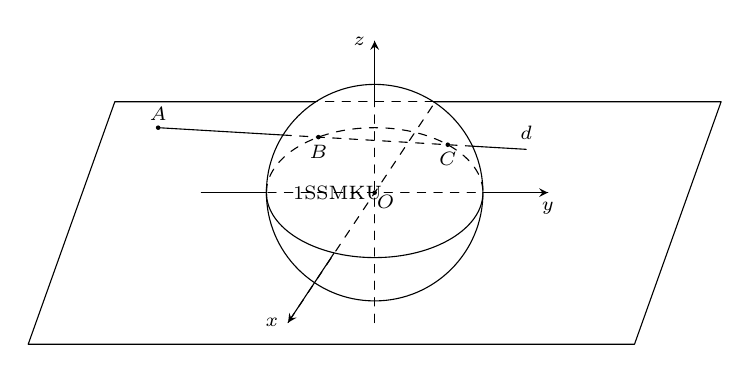
\begin{tikzpicture}[>=stealth,line join=round,font=\scriptsize,line cap=round,scale=0.55]
    %hidden: TV025
			%Gọi điểm
			\path
				(-6,2.1) coordinate (M)
				(8,2.1) coordinate (N)
				(-8,-3.5) coordinate (Q)
				($(N)+(Q)-(M)$) coordinate (P)
				(0,0) coordinate (O)
				($(O)-(2.5,0)$) coordinate (H)
				(-5,1.5) coordinate (A)
				(3.5,1) coordinate (D);
			%Vẽ đường thẳng d
			\path[name path=d] (A)--(D) node[above]{$ d $};
			\path[name path=(C)] (O) circle (2.5 cm);
			\path[name path=(E)] (O) ellipse (2.5 cm and 1.5 cm);
			\path[name intersections={of=d and (E),by={C,B}}];
			\path[name intersections={of=d and (C),by={I,J}}];
			\draw (A)--(J)
				(I)--(D);
			\draw[dashed] (J)--(I);
			%Vẽ hình cầu
			\draw
				(H) arc (180:0:2.5)
				(H) arc (-180:0:2.5 cm and 1.5 cm);
			\draw[dashed,thin] (H) arc (180:0:2.5 cm and 1.5 cm);
			\draw[thin] (H) arc (-180:0:2.5);
			%Vẽ mặt phẳng
			\path[name path=MN] (M)--(N);
			\path[name intersections={of=MN and (C),by={E,F}}];
			\draw[dashed] (E)--(F);
			\draw (M)--(F)
				(E)--(N)--(P)--(Q)--(M);
			%Vẽ hệ trục Oxyz
			\draw[dashed,->] ($(O)+(2*2/3,3*2/3)$)--($(O)-(2,3)$) node[left]{$ x $}; \draw (-0.94,-1.4)--(-2,-3);
			\draw[dashed,->] ($(O)-(4,0)$)--($(O)+(4,0)$) node[below]{$ y $}; \draw (-4,0)--(-2.5,0)
			(2.5,0)--(4,0);
			\draw[dashed,->] ($(O)-(0,3)$)--($(O)+(0,3.5)$) node[left]{$ z $}; \draw (0,2)--(0,3.5);
			%Đặt tên
			\foreach \i/\g in {O/-40,B/-90,C/-90,A/90}{\fill (\i) circle (1.5pt)
			($(\i)+(\g:3.3mm)$) node[scale=1]{$\i$};}
    \node at (0,0){\href{1SSMKU}{\tiny \phantom{1SSMKU}}};
		\end{tikzpicture}
	\end{center}
	\choiceTF
		{\True Phương trình tham số của đường thẳng $d$ là $\heva{&x=-688+91t\\&y=-185+75t\\&z=8}$, ($t\in\mathbb{R}$)}
		{\True Vị trí sớm nhất mà máy bay xuất hiện trên màn hình ra đa là điểm $B(-415;40;8)$}
		{Khoảng cách giữa vị trí đầu tiên và vị trí cuối cùng mà máy bay di chuyển trong phạm vi theo dõi của hệ thống quan sát là $497{,}54$ (km) (làm tròn kết quả đến hàng trăm theo đơn vị km)}
		{Máy bay đang chuyển động theo đường thẳng $d$ đến vị trí điểm $M(-500;100;100)$. Vị trí này nằm ngoài vùng kiểm soát không lưu của đài kiểm soát không lưu sân bay}
	\loigiai{
		\begin{itemchoice}
			\itemch Đường thẳng $d$ đi qua điểm $A(-688;-185;8)$ và có vectơ chỉ phương $\overrightarrow{u}=(91;75;0)$ nên phương trình tham số của $d\colon\heva{&x=-688+91t\\&y=-185+75t\\&z=8}(t\in\mathbb{R})$.
			\itemch Gọi $M(x;y;z)$ là vị trí của máy bay trên đường thẳng $d$.\\
			Ta có $M(-688+91t;-185+75t; 8)$.\\
			Máy bay xuất hiện trên màn hình ra đa khi
			\allowdisplaybreaks
			\begin{eqnarray*}
				OM\le 417&\Leftrightarrow& OM^2\le 417^2=173\,889\\
				&\Leftrightarrow& (-688+91t)^2+(-185+75t)^2+8^2\le 173\,889\\
				&\Leftrightarrow& (8\,281t^2-125\,216t+473\,344)+(5\,625t^2-27\,750t+34\,225)+64\le 173\,889\\
				&\Leftrightarrow& 13\,906t^2-152\,966t+507\,633\le 173\,889\\
				&\Leftrightarrow& 13\,906t^2-152\,966t+333\,744\le 0\\
				&\Leftrightarrow& 3\le t\le 8.
			\end{eqnarray*}
			Vị trí sớm nhất ứng với giá trị $t$ nhỏ nhất, tức là $t=3$.\\
			Khi đó tọa độ điểm $B$ là $\heva{&x=-688+91\cdot3=-415\\&y=-185+75\cdot3=40\\&z=8}\Rightarrow B(-415;40;8)$.
			\itemch Vị trí cuối cùng trong phạm vi theo dõi ứng với $t=8$.\\
			Khi đó tọa độ điểm $C$ là $\heva{&x=-688+91\cdot 8=40\\&y=-185+75\cdot 8=415\\&z=8}\Rightarrow C(40;415;8)$.\\
			Khoảng cách giữa hai vị trí này là
			\[BC=\sqrt{\left(40-(-415)\right)^2+(415-40)^2+(8-8)^2}=\sqrt{455^2+375^2}\approx 589{,}62\;(\text{km}).\]
			\itemch Xét điểm $M(-500;100;100)$.\\
			Ta thấy mọi điểm nằm trên đường thẳng $d$ đều có cao độ $z=8$, trong khi điểm $M$ có cao độ $z=100$.\\
			Do đó điểm $M$ không thuộc quỹ đạo bay (đường thẳng $d$).
		\end{itemchoice}
	}
\end{ex}

\begin{ex}%[VN-MT-8]%[2-D6B1-SO-1-2425, Nguyễn Quang Hiệp]%[2D6V1-2]
 Một viện bỏng có $2$ nguyên nhân chính là bỏng nhiệt và bỏng hóa chất, lần lượt chiếm $70 \%$ và $30 \%$ số bệnh nhân. Trong số bệnh nhân bị bỏng nhiệt, $30 \%$ có biến chứng, và trong số bệnh nhân bị bỏng hóa chất, $50 \%$ có biến chứng. Rút ngẫu nhiên một bệnh án, hãy đánh giá các phát biểu sau là đúng hay sai.
 \choiceTF
 {\True Xác suất của bỏng nhiệt bị biến chứng là $0{,}3$}
 {\True Xác suất của bỏng hóa chất bị biến chứng là $0{,}5$}
 { Xác suất của bệnh án bị biến chứng là $32 \%$}
 {\True Bệnh án rút ra bị biến chứng, xác suất bệnh án đó do bỏng nhiệt là $\dfrac{7}{12}$}
 \loigiai{
 Gọi
 \begin{itemize}
 \item $A$ là biến cố ``bệnh nhân bị bỏng nhiệt''.
 \item $B$ là biến cố ``bệnh nhân bị bỏng hóa chất''.
 \item $C$ là biến cố ``bệnh nhân bị biến chứng''.
 \end{itemize}
 Khi đó $\mathrm{P}(A)=0{,}7$; $\mathrm{P}(B)=0{,}3$. 
 \begin{itemchoice}
 \itemch \textbf{Đúng}.\\ Xác suất của bỏng nhiệt bị biến chứng là 
 \[
 \mathrm{P}\left(C \mid A\right) = 0{,}3.
 \]
 \itemch \textbf{Đúng}.\\ Xác suất của bỏng hóa chất bị biến chứng là
 \[
 \mathrm{P}\left(C \mid B\right) = 0{,}5.
 \]
 \itemch \textbf{Sai}.\\ Xác suất của biến cố bệnh nhân bị biến chứng là
 \allowdisplaybreaks
 \begin{eqnarray*}
 \mathrm{P}(C) &=& \mathrm{P}(C \mid A) \cdot \mathrm{P}(A) + \mathrm{P}\left(C \mid B\right) \cdot \mathrm{P}(B)\\
 &=& 0{,}3 \cdot 0{,}7 + 0{,}5 \cdot 0{,}3 = 0{,}21 + 0{,}15 = 0{,}36.
 \end{eqnarray*}
 \itemch \textbf{Đúng}.\\
 Ta có $\mathrm{P}\left(AC\right) = \mathrm{P}(A) \cdot \mathrm{P}(C|A) = (0{,}7)(0{,}3) = 0{,}21$.\\
 Khi đó bệnh án rút ra bị biến chứng, xác suất bệnh án đó do bỏng nhiệt là \[
 \mathrm{P}\left(A \mid C\right) = \dfrac{\mathrm{P}\left(AC\right)}{\mathrm{P}(C)} = \dfrac{0{,}21}{0{,}36}= \dfrac{7}{12}.
 \]
 \end{itemchoice}
 }
\end{ex}
\vspace{0.5cm}

\begin{center}
\noindent\textbf{\large PHẦN III. Câu hỏi trắc nghiệm trả lời ngắn.}
\\ \textit{Thí sinh trả lời từ câu 1 đến câu 6. Thí sinh điền đáp số vào ô trống tương ứng.}
\end{center}
\setcounter{ex}{0}

\begin{ex}%[VN-MT-8]%[2-D4B2-SO-5-2425, Đặng Anh Thư]%[2D4H2-2]
 Cho $\displaystyle\int\limits_{1}^{3} \dfrac{x+2}{x} \mathrm{\,d}x=a+ b \ln c$, với $a$, $b$, $c \in \mathbb{Z}$ và $b$ là số nguyên tố. Tính tổng $S=a+b+c$.
 \par
 \shortans{7}
 
 \loigiai{ Ta có $\displaystyle\int\limits_{1}^{3} \dfrac{x+2}{x} \mathrm{\,d}x=\displaystyle\int\limits_{1}^{3} \left( 1+ \dfrac{2}{x}\right) \mathrm{\,d}x=\left( x+ 2 \ln \left|x \right| \right)\biggr|_1^3=\left(3+ 2 \ln3 \right) -\left(1+\ln1 \right)=2+2\ln3$.\\
 Do đó $a=2$, $b=2$, $c=3$. Vậy $a+b+c=2+2+3=7$.
 }
\end{ex}

\begin{ex}%[VN-MT-8]%[2-D4B3-SO-9-2425, Khổng Xuân Thạnh]%[2D4V3-1]
 Cho hình phẳng $(H)$ giới hạn bởi các đường $y=\left|x^2-1\right|$ và $y=k$, với $0<k<1$ sao cho diện tích hình phẳng $(H)$ gấp hai lần diện tích hình phẳng được kẻ sọc ở hình vẽ sau. Khi đó $k=\sqrt[m]{n}-p$ (trong đó $m,n,p$ là số nguyên dương và $m,n$ là hai số nguyên tố cùng nhau) thì giá trị của $m+n+p$ bằng bao nhiêu?
 \begin{center}
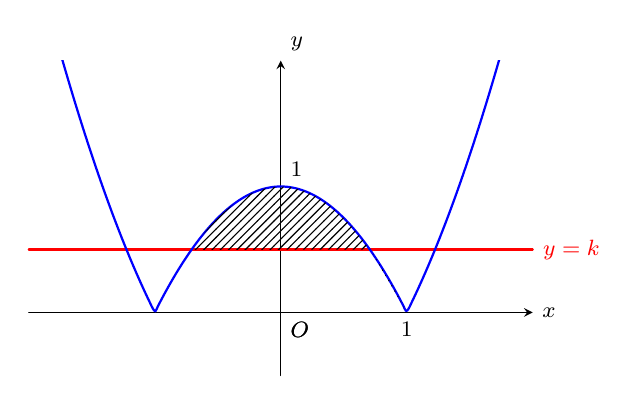
\begin{tikzpicture}[scale=1, font=\footnotesize, line join=round, line cap=round, >=stealth, x=1.6cm, y=1.6cm]
 % Axes
 \def\k{0.5}
 \draw[->] (-2,0) -- (2,0) node[right] {$x$};
 \draw[->] (0,-0.5) -- (0,2) node[above right] {$y$};
 \draw (0,0) node [below right] {$O$};
 \draw (0,0) node [below right] {$O$};
 \draw (1,0) node[below]{$1$} (0,1)node[above right]{$1$};
 \draw[red,thick] (-2,\k) -- (2,\k) node[right] {$y=k$};
 \begin{scope}
 \clip (-2,-0.5) rectangle (2,2);
 \draw[domain=-2:2,smooth,samples=200,variable=\x,blue,thick] plot ({\x},{abs(\x*\x-1)});
 \fill[pattern=north east lines] 
 (0.71,0.5) -- 
 plot[domain=-0.71:1] (\x,{abs(\x*\x-1)});
 \end{scope}
\end{tikzpicture}
 \end{center}
\shortans{8}
\loigiai{
 Ta có $y=\left|x^2-1\right|\Leftrightarrow \heva{x^2-1\quad &\text{khi}&\, x\geq0\\ -x^2+1\quad &\text{khi}&\, x<0.}$\\
Do đồ thị nhận trục $Oy$ làm trục đối xứng nên yêu cầu bài toán trở thành:
Diện tích hình phẳng giới hạn bởi $y=1-{{x}^{2}},y=k,x=0$ bằng diện tích hình phẳng giới hạn bởi $y=1-x^2$, $y=x^2-1$, $y=k$ khi $x>0$. Do đó ta có
\allowdisplaybreaks \begin{eqnarray*}
&&\displaystyle\int\limits_0^{\sqrt{1-k}} \left(1-x^2-k\right)\mathrm{\,d}x
=\displaystyle\int\limits_{\sqrt{1-k}}^{1}{\left(k-1+x^2\right)}\mathrm{\,d}x+\displaystyle\int\limits_1^{\sqrt{1+k}}\left(k-x^2+1\right)\mathrm{\,d}x\\
&\Leftrightarrow& \left(1-k\right)\sqrt{1-k}-\dfrac{1}{3}\left(1-k\right)\sqrt{1-k}=\dfrac{1}{3}-\left(1-k\right)-\dfrac{1}{3}\left(1-k\right)\sqrt{1-k}+\left(1-k\right)\sqrt{1-k} \\ 
&+&\left( 1+k \right) \sqrt{1+k}-\dfrac{1}{3}\left(1+k\right)\sqrt{1+k}-\left(1+k\right)+\dfrac{1}{3} \\ 
&\Leftrightarrow& \dfrac{2}{3}\left(1+k\right)\sqrt{1+k}=\dfrac{4}{3}\\
&\Leftrightarrow& \left(\sqrt{1+k}\right)^3=2\\
&\Leftrightarrow& k=\sqrt[3]{4}-1.
\end{eqnarray*}
Theo đề $k=\sqrt[m]{n}-p$, khi đó $m=3$, $n=4$, $p=1$.\\
Vậy $m+n+p=3+4+1=8$.
}
\end{ex}

\begin{ex}%[VN-MT-8]%[2-H5B4-SO-12-2425, Nguyễn Khánh Trọng]%[2H5C3-2]
 Trong không gian với hệ trục tọa độ $Oxyz$, cho mặt cầu $(S)\colon (x-2)^2+(y-1)^2+(z-1)^2=9$ và điểm $M(x_0;y_0;z_0)$ thuộc mặt cầu $(S)$. Tìm giá trị nhỏ nhất của biểu thức $P=x_0+y_0+z_0$ (kết quả làm tròn đến hàng phần chục).\par
 \shortans{-1{,}2}
 \loigiai{
 Mặt cầu $(S)$ có tâm $I(2;1;1)$ và bán kính $R=3$.\\
 Gọi mặt phẳng $(\alpha)\colon x+y+z-P=0$.\\
 Suy ra $M(x_0;y_0;z_0)\in (\alpha)$. Do đó $M\in (\alpha)\cap (S)$.\\
 Mặt phẳng $(\alpha)$ và mặt cầu $(S)$ có giao điểm khi và chỉ khi
 \allowdisplaybreaks
 \begin{eqnarray*}
 &&\mathrm{d}\big(I,(\alpha)\big)\le R \\
 &\Leftrightarrow& \dfrac{|2+1+1-P|}{\sqrt{1+1+1}}\le3\\ &\Leftrightarrow& |4-P|\le 3\sqrt{3}\\
 &\Leftrightarrow& -3\sqrt{3}\le 4-P\le 3\sqrt{3}\\
 &\Leftrightarrow& 4-3\sqrt{3}\le P\le 4+3\sqrt{3}.
 \end{eqnarray*}
 Vậy $P_{\min}=4-3\sqrt{3}$. Khi đó $x_0+y_0+z_0=4-3\sqrt{3}\approx -1{,}2$.
 }
\end{ex}

\begin{ex}%[VN-MT-8]%[2-H5B4-SO-12-2425, Nguyễn Khánh Trọng]%[2H5V3-2]
 Trong không gian với hệ trục tọa độ $Oxyz$, cho hai đường thẳng $d_1\colon \dfrac{x+1}{2}=\dfrac{y-3}{-1}=\dfrac{z+2}{1}$; $d_2\colon \dfrac{x-1}{-1}=\dfrac{y-2}{1}=\dfrac{z+2}{2}$. Mặt cầu $(S)$ tiếp xúc với $d_1$ tại điểm có hoành độ bằng $1$ và có tâm nằm trên đường thẳng $d_2$. Phương trình mặt cầu $(S)$ có dạng
 $(x-a)^2+(y-b)^2+(z-c)^2=R^2$, khi đó $a+2b+3c$ bằng bao nhiêu?\par
 \shortans{-8}
 \loigiai{
 Gọi $A\in d_1$ với $x_A=1\Rightarrow y_A=2$ và $z_A=-1$. Suy ra $A(1;2;-1)$.\\
 Gọi mặt cầu $(S)$ có tâm $I$.\\
 Ta có $I\in d_2\colon\heva{&x=1-t\\&y=2+t\\&z=-2+2t}\Rightarrow I(1-t;2+t;-2+2t)$. Khi đó $\overrightarrow{AI}=(-t;t;-1+2t)$.\\
 Vì $(S)$ tiếp xúc với $d_1$ tại $A$ nên $\overrightarrow{AI}\perp \overrightarrow{u}_1$ với $\overrightarrow{u}_1=(2;-1;1)$ là vectơ chỉ phương của $d_1$.\\
 Suy ra $\overrightarrow{AI}\cdot\overrightarrow{u}_1=0\Leftrightarrow -2t-t-1+2t=0\Leftrightarrow t=-1$.\\
 Do đó $I(2;1;-4)$. Vậy $a+2b+3c=2+2\cdot1+3\cdot(-4)=-8$.
 }
\end{ex}

\begin{ex}%[Dự án 5C31SL-VN-MT-11]%[2-KS-13-SoHaiDuong-2025,TV030]%[2D6V1-3]
	Hiện nay, nước ta đang trong quá trình tinh gọn bộ máy và thực hiện nghị quyết không tổ chức công an cấp huyện. Do vậy, trong đợt điều động cán bộ công an từ huyện về công tác tại cơ sở hoặc công tác tại công an tỉnh, phòng tổ chức cán bộ nhận thấy rằng: có $60\%$ cán bộ có nguyện vọng về công tác tại cơ sở là các xã vùng sâu vùng xa, số còn lại nguyện vọng về công tác tại công an tỉnh.
	\begin{itemize}
		\item Trong số cán bộ có nguyện vọng về công tác tại cơ sở thì $70\%$ có trình độ đại học và $30\%$ có trình độ trung cấp.
		\item Trong số cán bộ có nguyện vọng về công an tỉnh thì $80\%$ có trình độ đại học và $20\%$ có trình độ trung cấp.
	\end{itemize}
	Tuy nhiên, năng lực công tác cũng là một yếu tố quan trọng. Dựa trên hồ sơ đánh giá năng lực:
	\begin{itemize}
		\item Trong số cán bộ có nguyện vọng về cơ sở thì tỷ lệ cán bộ được đánh giá có năng lực \lq\lq Tốt\rq\rq\, trở lên với trình độ đại học là $60\%$ và trình độ trung cấp là $30\%$.
		\item Trong số cán bộ có nguyện vọng về công tác tại công an tỉnh thì tỷ lệ cán bộ được đánh giá có năng lực \lq\lq Tốt\rq\rq\, trở lên với trình độ đại học là $85\%$ và trình độ trung cấp là $25\%$.
	\end{itemize}
	Chọn ngẫu nhiên một cán bộ công an. Tính xác suất để cán bộ này vừa có trình độ đại học, vừa được đánh giá có năng lực \lq\lq Tốt\rq\rq\, và có nguyện vọng về công tác tại cơ sở là các xã vùng sâu vùng xa (kết quả làm tròn đến hàng phần trăm).
	\par
	\shortans{0,25}
	\loigiai{
		Gọi $A$ là biến cố: \lq\lq Cán bộ có nguyện vọng về công tác tại cơ sở là các xã vùng sâu vùng xa\rq\rq.\\
		Khi đó, $\overline{A}$ là biến cố: \lq\lq Cán bộ có nguyện vọng về công tác tại công an tỉnh\rq\rq.\\
		Gọi $B$ là biến cố: \lq\lq Cán bộ có trình độ đại học\lq\lq.\\
		Khi đó, $\overline{B}$ là biến cố: \lq\lq Cán bộ có trình độ trung cấp\rq\rq.\\
		Gọi $C$ là biến cố: \lq\lq Cán bộ được đánh giá là có năng lực \lq\lq Tốt\rq\rq\, trở lên\rq\rq.\\
		Ta có sơ đồ cây như sau:
		\begin{center}
			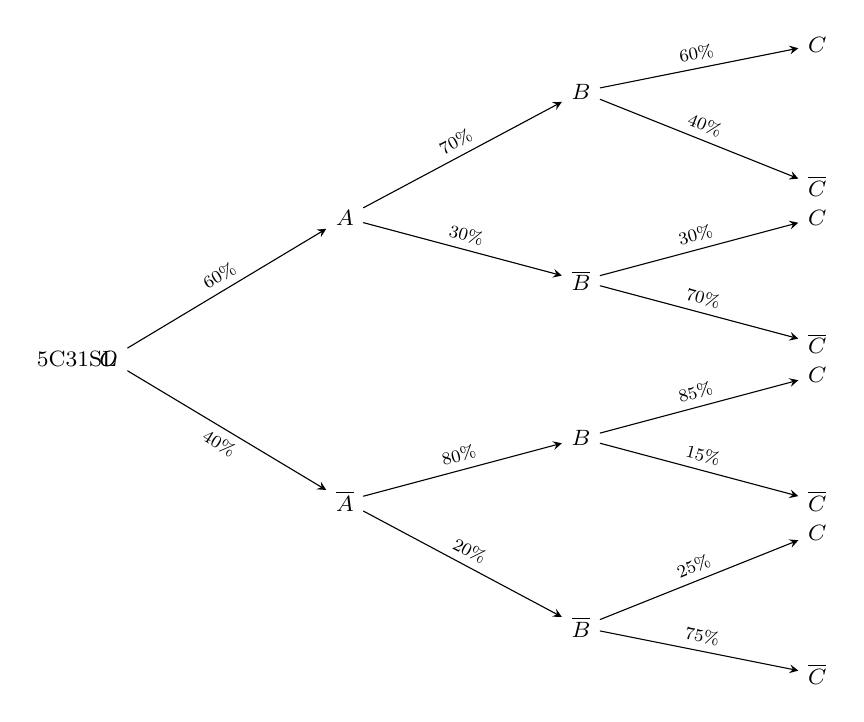
\begin{tikzpicture}[->,>=stealth,line join=round,line cap=round,font=\footnotesize,scale=1]
    %hidden: TV021
				\def\xmot{3}
				\def\xhai{6}
				\def\xba{9}
				\node (O) at (0,0){$O$};
				\node (B) at (\xmot,1.8){$A$};
				\node (B1) at (\xmot,-1.8){$\overline{A}$};
				\node (BA) at (\xhai,3.4){$B$};
				\node (BA1) at (\xhai,1){$\overline{B}$};
				\node (B1A) at (\xhai,-1){$B$};
				\node (B1A1) at (\xhai,-3.4){$\overline{B}$};
				\node (C1) at (\xba,4){$C$};
				\node (C2) at (\xba,2.2){$\overline{C}$};
				\node (C3) at (\xba,1.8){$C$};
				\node (C4) at (\xba,0.2){$\overline{C}$};
				\node (C5) at (\xba,-0.2){$C$};
				\node (C6) at (\xba,-1.8){$\overline{C}$};
				\node (C7) at (\xba,-2.2){$C$};
				\node (C8) at (\xba,-4){$\overline{C}$};
				\foreach \x/\y/\p/\l in 
				{O/B/above/$60\%$,
					B/BA/above/$70\%$,
					B/BA1/above/$30\%$,
					O/B1/below/$40\%$,
					B1/B1A/above/$80\%$,
					B1/B1A1/above/$20\%$,
					BA/C1/above/$60\%$, BA/C2/above/$40\%$,
					BA1/C3/above/$30\%$, BA1/C4/above/$70\%$,
					B1A/C5/above/$85\%$, B1A/C6/above/$15\%$,
					B1A1/C7/above/$25\%$, B1A1/C8/above/$75\%$
				}
				{
					\draw[->] (\x)--(\y)node[midway,\p,scale=0.8,sloped]{\l};
				}
    \node at (0,0){\href{5C31SL}{\tiny \phantom{5C31SL}}};
			\end{tikzpicture}
		\end{center}
		Từ đó, xác suất để cán bộ này vừa có trình độ đại học, vừa được đánh giá có năng lực \lq\lq Tốt\rq\rq\,và có nguyện vọng về công tác tại cơ sở là các vùng sâu vùng xa là
		\[\mathrm{P}(ABC)=0{,}6\cdot 0{,}7\cdot 0{,}6=0{,}252\approx 0{,}25.\]
	}
\end{ex}

\begin{ex}%[VN-MT-8]%[2-D6B3-SO-9-2425, Nguyễn Trường Vinh]%[2D6C2-3]
Một nhà máy sản xuất bóng đèn có tỉ lệ bóng đèn đạt tiêu chuẩn là $80\%$. Trước khi xuất ra thị trường, mỗi bóng đèn đều được kiểm tra chất lượng. Vì sự kiểm tra không thể tuyệt đối hoàn hảo nên tỉ lệ công nhận một bóng đèn đạt tiêu chuẩn là $0{,}9$ và tỉ lệ loại bỏ một bóng hỏng là $0{,}95$. Hãy tính tỉ lệ bóng đạt tiêu chuẩn sau khi qua khâu kiểm tra chất lượng (kết quả làm tròn đến hàng đơn vị tính theo $\%$).
\par
\shortans{73}
\loigiai{
Gọi $A$ là biến cố ``Bóng đèn đạt tiêu chuẩn sau khi qua khâu kiểm tra''.\\
Gọi $B$ là biến cố ``Bóng đèn đạt tiêu chuẩn khi sản xuất''.\\
Gọi $\overline{B}$ là biến cố ``Bóng đèn không đạt tiêu chuẩn khi sản xuất''.\\
Khi đó, ta có $\mathrm{P}(B) = \dfrac{4}{5}$, $\mathrm{P} \left(\overline{B}\right) = \dfrac{1}{5}$, $\mathrm{P}(A\mid B) = \dfrac{9}{10}$ và $\mathrm{P} \left(A\mid \overline{B} \right) =1-0{,}95= \dfrac{1}{20}$.\\
Ta có xác suất bóng đèn đạt tiêu chuẩn sau khi qua khâu kiểm tra chất lượng là
\begin{align*}
\mathrm{P}(A) &= \mathrm{P}(B)\cdot \mathrm{P}(A\mid B) + \mathrm{P} \left(\overline{B}\right)\cdot \mathrm{P} \left(A\mid \overline{B} \right)\\
&= \dfrac{4}{5}\cdot \dfrac{9}{10} + \dfrac{1}{5} \cdot \dfrac{1}{20} \approx 0{,}73.
\end{align*}
Vậy tỉ lệ bóng đạt tiêu chuẩn sau khi qua khâu kiểm tra chất lượng là $73\%$.
}
\end{ex}
\vspace{0.5cm}



\end{document}
